\documentclass[conference]{IEEEtran}
\IEEEoverridecommandlockouts

\usepackage{amsmath,amssymb,amsfonts}
\usepackage{graphicx}
\usepackage{textcomp}
\usepackage{booktabs}
\usepackage{tabularx}
\usepackage{url}

\begin{document}

\title{ANESTHESIA DOSE CALCULATION AND SAFETY SUPPORT SYSTEM}

\author{
\IEEEauthorblockN{Dr.~Sowbahgya~M~P\IEEEauthorrefmark{1}, Mohammed~Shazan\IEEEauthorrefmark{2}, Mohan~Gowda~V~C\IEEEauthorrefmark{3}, and Puneeth~S~V\IEEEauthorrefmark{4}}
\IEEEauthorblockA{\IEEEauthorrefmark{1}Associate Professor, \IEEEauthorrefmark{2}\IEEEauthorrefmark{3}\IEEEauthorrefmark{4}Student\\
Department of Computer Science and Engineering, K.S. Institute of Technology\\
Visvesvaraya Technological University, Bengaluru, Karnataka, India\\
Email: \IEEEauthorrefmark{1}sowbahgya.mp@gmail.com, \IEEEauthorrefmark{2}mohammedshazan888@gmail.com, \\
\IEEEauthorrefmark{3}mohangowda4983@gmail.com, \IEEEauthorrefmark{4}punithsv948@gmail.com}
}

\maketitle

\begin{abstract}
Perioperative patient management demands meticulous pharmacological planning, continuous hemodynamic surveillance, and timely clinical decision-making to mitigate intraoperative instability. Conventional perioperative workflows place substantial cognitive load upon anesthesiologists, who must synthesize fragmented physiological signals, calculate customized medication dosages, and track fluid shifts under strict time constraints. This paper presents \textbf{Anesth AI}, an integrated, human-in-the-loop clinical decision-support prototype designed for perioperative anesthesia management and patient safety. The platform integrates four benchmark biomedical databases---VitalDB, the MIT-BIH Arrhythmia Database, MIMIC-IV-ED v2.2, and MIMIC-IV v3.1---to evaluate ten operational clinical prediction tasks across hemodynamic instability, electrophysiological dysrhythmia, surgical hemorrhage, intravenous volume response, emergency triage acuity, intensive care admission, and in-hospital mortality. A strict three-way patient- and record-grouped validation protocol ($70\%$ training, $15\%$ validation, $15\%$ frozen test) was enforced, eliminating target leakage and restricting preprocessing transformations exclusively to training sets. Across frozen held-out cohorts, benchmark models demonstrate strong discriminatory performance: ICU Admission (ClinicalGRU: AUROC $0.8814$), Fluid Recommendation (LightGBM: AUROC $0.8687$), Blood Loss (ClinicalLSTM: AUROC $0.8349$), Hypoxia (HistGradientBoosting: AUROC $0.9047$), and Emergency Severity (CatBoost: Sensitivity $78.78\%$). Authentic revalidation on all 48 MIT-BIH records ($109,494$ beats) resolved an earlier zero-positive test artifact, achieving an AUROC of $0.9414$ and sensitivity of $92.01\%$ on $5,843$ positive dysrhythmias ($N=17,029$). Anesth AI strictly decouples probabilistic machine learning from a deterministic physiological fluid engine, incorporates parameter-based dose calculation support, standardizes clinician-confirmed ASA Physical Status Classification, and embeds role-based access control with Emergency Break-Glass auditing. Operating strictly under clinician review, the system does not autonomously administer or titrate drugs, fluids, or mechanical ventilation.
\end{abstract}

\begin{IEEEkeywords}
\textbf{Artificial Intelligence, Clinical Decision Support, Anesthesia Dose Support, Perioperative Monitoring, Machine Learning, Deep Learning, Explainable AI, Patient Safety, Human-in-the-Loop}
\end{IEEEkeywords}

\section{Introduction}
Modern perioperative medicine is an intensely dynamic clinical domain wherein anesthesiologists continuously evaluate multi-parameter physiological streams, anticipate hemodynamic collapse, titrate potent pharmacologic agents, and maintain surgical safety protocols under acute time constraints. Adverse intraoperative events---such as sudden arterial hypotension, hypoxemia, cardiac dysrhythmias, and occult surgical hemorrhage---are directly associated with devastating postoperative morbidity, including acute myocardial injury, acute kidney injury, protracted intensive care unit hospitalization, and mortality.

In standard operative workflows, anesthesiologists rely upon threshold-based alerts emitted by isolated monitors. Although modern monitors track heart rate, blood pressures, and oxygen saturation, they emit frequent false-positive alarms, fail to model non-linear inter-parameter trajectories, and provide limited predictive foresight prior to decompensation. Anesthesiologists must mentally reconcile disparate data streams---preoperative medical histories, organ function laboratories, real-time waveforms, and cumulative surgical fluid balances---while manually computing drug dosages and hourly maintenance fluids. In prolonged or emergency trauma procedures, this manual burden induces severe cognitive fatigue, increasing the vulnerability to delayed recognition of critical physiological instability.

Recent advances in Artificial Intelligence and Machine Learning present significant potential for clinical decision support systems in perioperative care. By modeling complex physiological interactions across high-resolution clinical databases such as VitalDB, the MIT-BIH Arrhythmia Database, and MIMIC-IV, predictive models can alert clinicians to emergent risks before decompensation occurs. However, substantial methodological and translational limitations persist in the literature: data and target leakage due to random observation splitting, single-task siloing where models address isolated predictions without full perioperative continuity, and black-box automation risks that provoke clinical skepticism if mistaken for autonomous prescribing devices.

To address these clinical and computational challenges, this work introduces \textbf{Anesth AI}, an integrated, human-in-the-loop clinical decision-support prototype designed for personalized anesthesia management and perioperative patient safety. Engineered under strict biomedical guardrails, Anesth AI integrates multi-task machine learning, deterministic physiological fluid calculations, parameter-based dose calculation support, clinician-confirmed risk classification, Explainable AI (XAI), and dual-tier authentication with Emergency Break-Glass access.

The principal contributions of this work are: (1) Operational deployment of ten clinical prediction tasks spanning intraoperative hemodynamics, electrophysiology, hemorrhage, fluid response, emergency triage, and critical-care survival across four benchmark databases; (2) Enforced three-way patient- and record-grouped splitting with complete purging of target-defining predictors and restriction of scalers to training partitions; (3) Authentic Arrhythmia task revalidation across all 48 MIT-BIH records ($109,494$ beats) correcting an earlier parsing issue; (4) Transparent decoupling of probabilistic ML recommendations from a deterministic physiological fluid calculation engine based on Holliday-Segar basal requirements, Estimated Blood Volume, and ATLS hemorrhage staging; (5) Clinician-confirmed ASA Physical Status Classification, structured WHO safety checklists, parameter-based dose calculation support, and objective alert semantics; and (6) Centralized Role-Based Access Control across six clinical roles paired with an audited Emergency Break-Glass protocol.

\section{Literature Survey}
The integration of machine learning into perioperative medicine has progressed rapidly from early single-variable prototypes toward comprehensive, multi-modal clinical decision-support systems, as reflected in recent peer-reviewed literature published from 2024 to 2026.

In a comprehensive systematic review and meta-analysis of perioperative anesthetic management, Shimada et al. (2024) evaluated 18 randomized and observational trial cohorts ($N=2,150$) utilizing artificial intelligence-guided hemodynamic and hypnotic interventions. The authors reported that computer-assisted decision support significantly reduced the cumulative duration of intraoperative arterial hypotension and improved bispectral index maintenance compared to routine clinical practice; however, marked protocol heterogeneity and the absence of standardized surgical fluid accounting were highlighted as key translational barriers.

In pharmacological dosage modeling, Hu et al. (2024) developed deep neural network architectures using tabular clinical parameters, including age, weight, and surgical classification on a surgical cohort ($N=120$). Their deep model reduced mean absolute dosage error compared to conventional empirical rules; however, the formulation was restricted to static pre-induction variables, lacking integration with continuous intraoperative vital telemetry, fluid balances, and organ-function safety flags.

Synthesizing contemporary trends across clinical anesthesiology, Shu et al. (2025) reviewed machine learning applications across preoperative risk stratification, intraoperative depth-of-anesthesia monitoring, and postoperative intensive care triage. The authors demonstrated that machine learning architectures consistently outperform static risk indices in forecasting circulatory collapse, but identified that over 80\% of existing models function in isolated silos without end-to-end perioperative continuity or unified clinical interfaces.

Examining safety governance and clinical trust, Fei et al. (2025) reviewed artificial intelligence implementations in anesthesia and perioperative medicine across multi-institutional datasets. The investigation emphasized that advisory decision-support frameworks maintain clinician trust and diagnostic vigilance compared to fully autonomous proposals, while noting that emergency bypass mechanisms and audited break-glass protocols remain almost entirely unaddressed in published academic systems.

In a multi-center observational trial of clinical decision support, Bellini et al. (2025) evaluated real-time predictive alerts across a surgical cohort ($N=1,420$). The authors reported a significant reduction in the duration of severe intraoperative hypotensive episodes; however, they observed high alert-fatigue rates and underscored that the omission of transparent physiological fluid accounting constrained overall clinical adoption.

Most recently, Chae et al. (2026) evaluated multi-modal physiological telemetry and deep sequence architectures across high-resolution operating room cohorts, demonstrating that sequential models anticipate critical hemodynamic collapse with a 10-minute lead time, while identifying substantial computational latency and the lack of structured surgical checklists as ongoing implementation challenges.

\begin{table*}[t]
\centering
\caption{Comparative Review of Recent Anesthesia AI Literature (2024--2026)}
\label{tab:lit_comparison}
\begin{tabularx}{\textwidth}{c p{3.2cm} p{2.8cm} p{3.2cm} p{2.8cm} p{3.5cm}}
\toprule
\textbf{Year} & \textbf{Methodological Approach} & \textbf{Data Source \& Cohort} & \textbf{Clinical Contribution} & \textbf{Clinical Outcome} & \textbf{Limitations} \\
\midrule
2024 & Systematic review and meta-analysis of AI interventions & 18 perioperative trial cohorts ($N=2,150$) & Evaluated AI-assisted hypnotic and hemodynamic management & Reduced hypotensive duration and improved bispectral maintenance & Trial protocol heterogeneity; lacks standardized intraoperative fluid balance. \\
2024 & Deep neural networks on tabular clinical variables & Single-center surgical cases ($N=120$) & Pre-induction personalized anesthesia dosage prediction & Reduced mean absolute dosage error vs. empirical guidelines & Static pre-induction only; lacks continuous telemetry and organ safety gates. \\
2025 & Comprehensive clinical review and algorithmic taxonomy & Published perioperative AI studies and trials & Mapped ML across risk stratification, dosing, and shock detection & Identified opportunities in multi-modal decision support & Isolated task silos; models lack end-to-end perioperative software continuity. \\
2025 & Review of decision support and patient safety frameworks & Multi-institutional clinical datasets & Analyzed human-in-the-loop workflows and alert governance & Affirmed CDSS trust over autonomous drug delivery systems & Evaluated architectures universally lacked audited emergency break-glass. \\
2025 & Multi-center decision-support trial analysis & Perioperative surgical cohort ($N=1,420$) & Real-time decision-support alerts for hemodynamic instability & Reduced duration of intraoperative hypotensive events & High alert fatigue; lacks integrated fluid tracking and override audit logs. \\
2026 & Multi-modal physiological deep sequence models & High-resolution operating room telemetry & Forecasting respiratory and circulatory decompensation & Anticipated critical collapse with 10-minute lead time & High computational inference latency; lacks standardized surgical checklists. \\
\bottomrule
\end{tabularx}
\end{table*}

\section{System Design and Architecture}
The clinical architecture of Anesth AI supports the perioperative continuum under strict human-in-the-loop governance across three clinical phases (Fig.~\ref{fig:arch} and Fig.~\ref{fig:workflow}). The system is engineered as an advisory clinical decision-support prototype; it does not autonomously prescribe, administer, or titrate drugs, intravenous fluids, or ventilator settings.

\begin{figure*}[t]
\centering
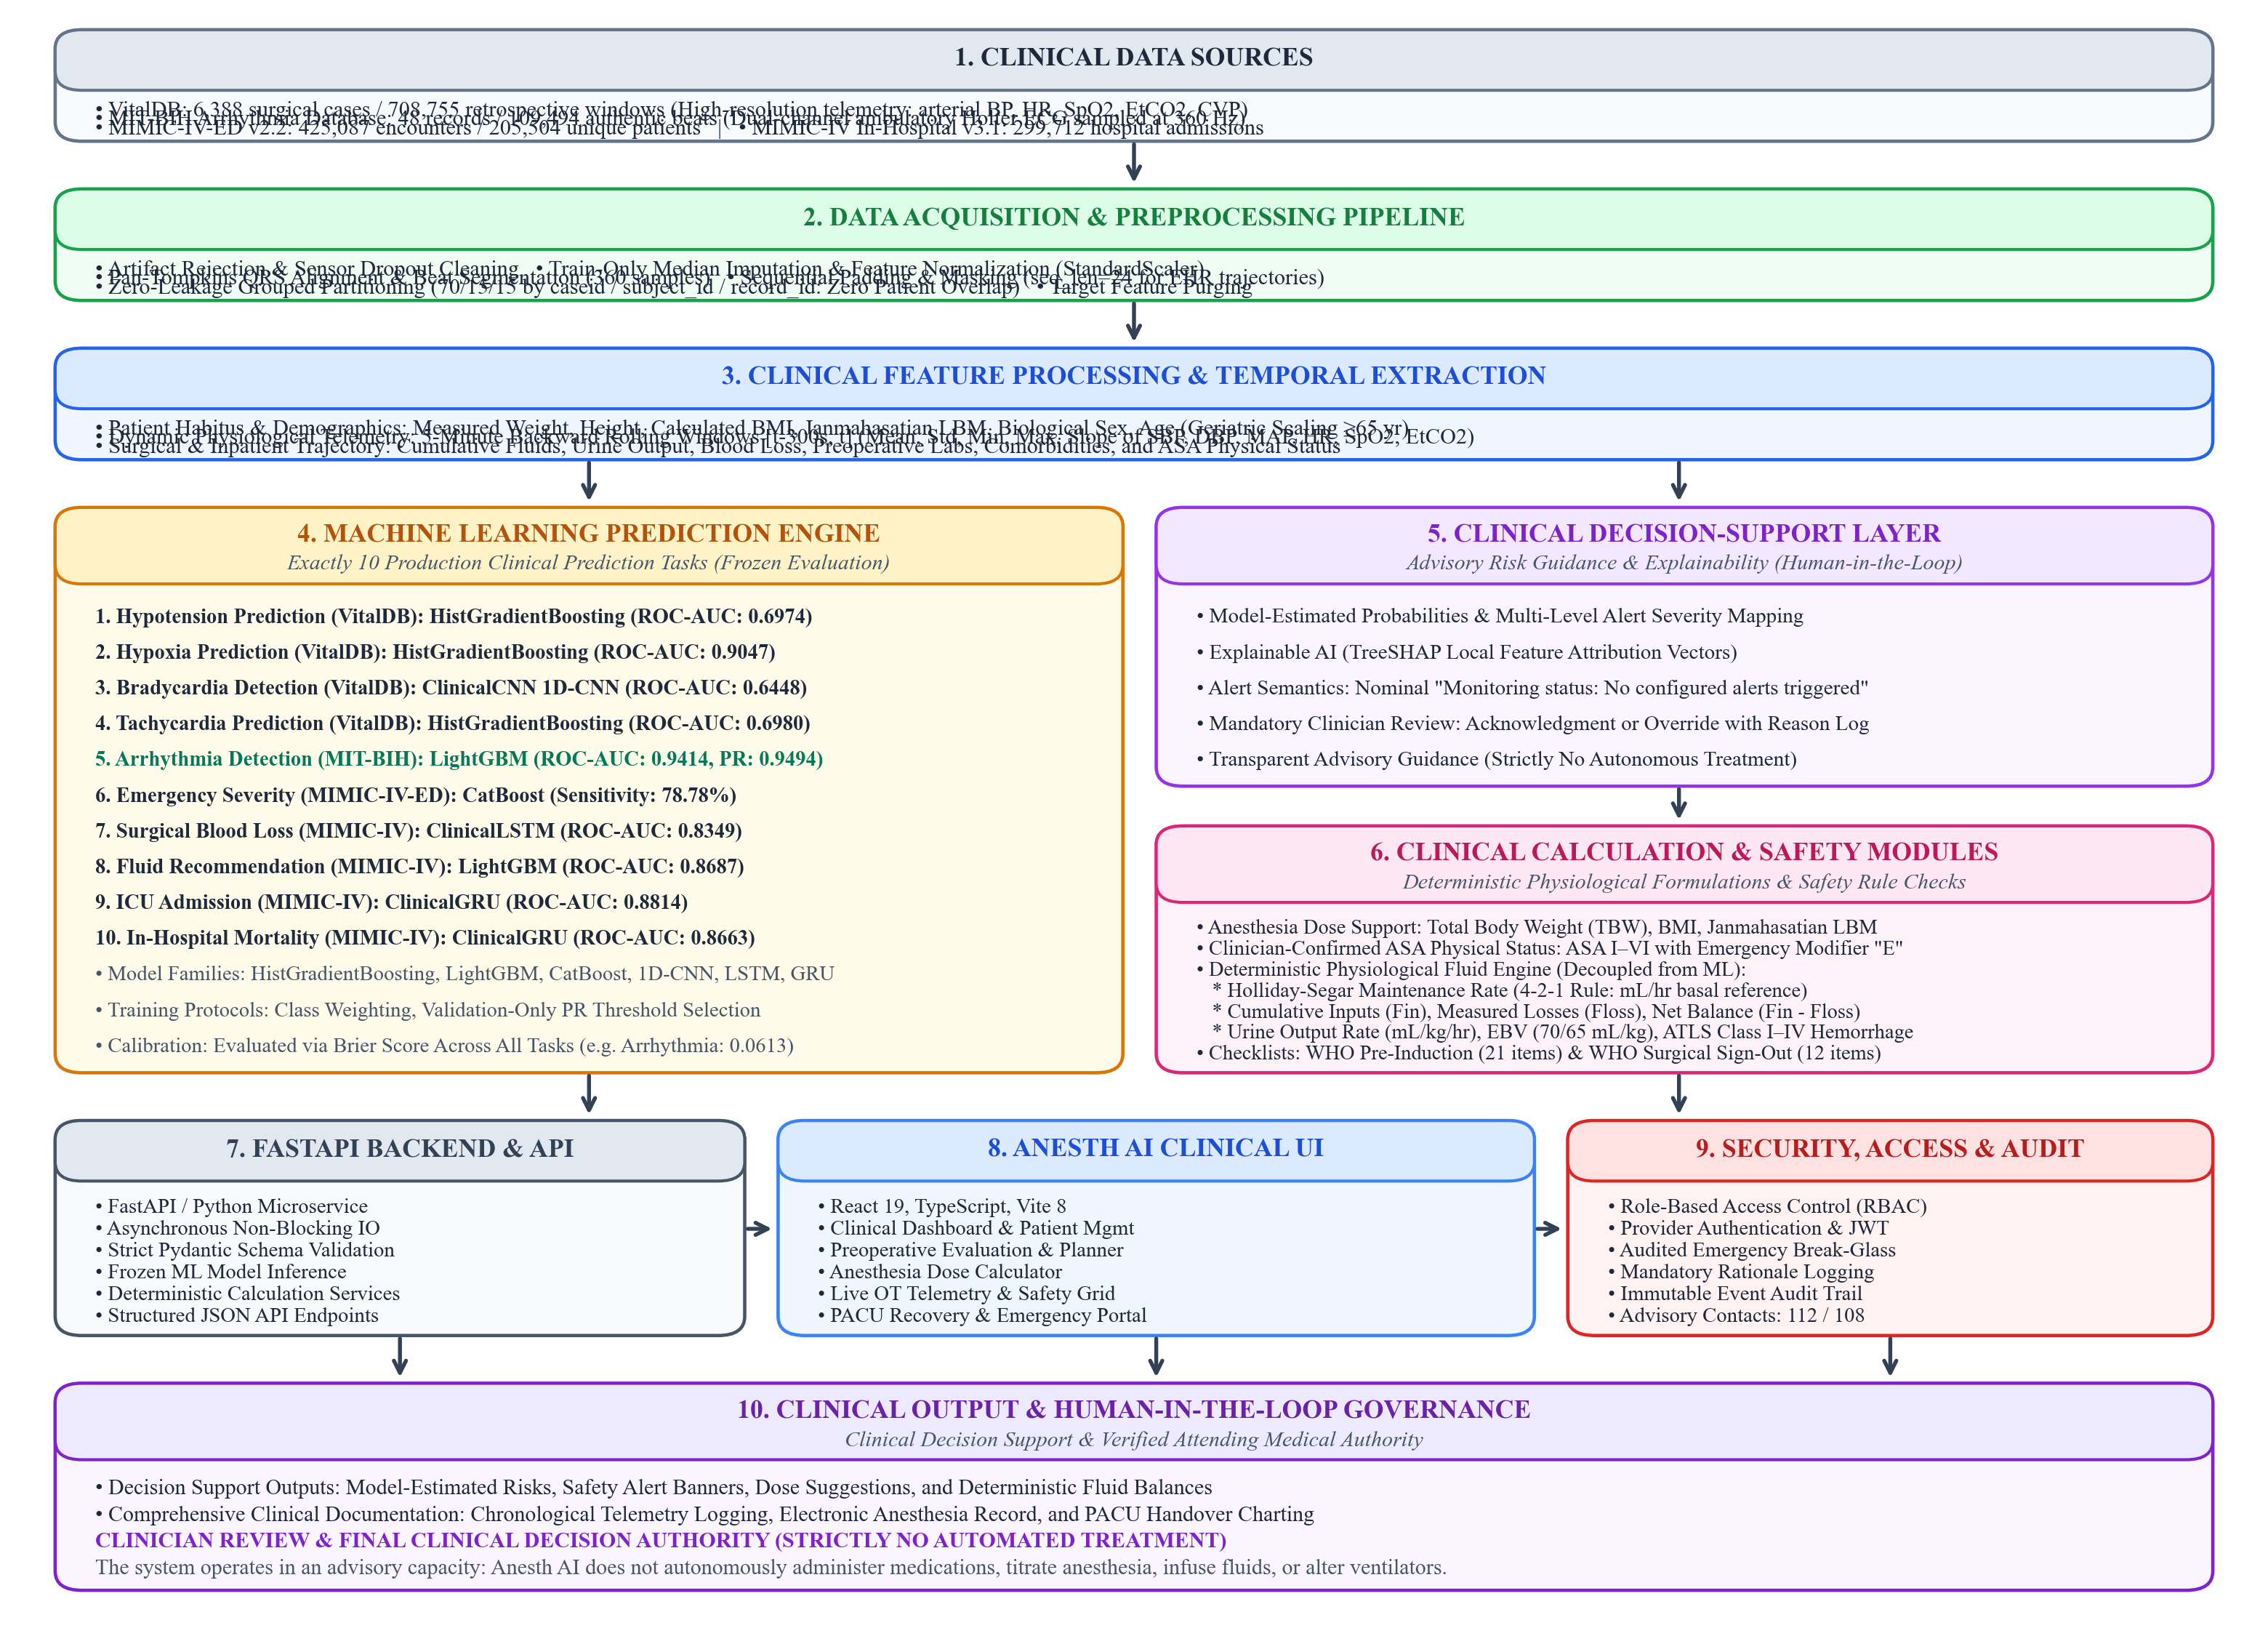
\includegraphics[width=0.73\textwidth]{figures_polished/fig1_architecture.png}
\caption{Current system architecture of Anesth AI.}
\label{fig:arch}
\end{figure*}

As illustrated in Fig.~\ref{fig:arch}, the platform comprises modular tiers coordinating clinical inputs, schema validation, predictive inference, deterministic arithmetic, and user interface components. The frontend is developed using React 19, TypeScript, and Vite 8, delivering responsive, low-latency clinical dashboards. The backend service is engineered in Python utilizing FastAPI, providing asynchronous execution with sub-50ms inference latency across all endpoints with Pydantic validation, JWT authentication, and structured error handling. Machine learning inference is orchestrated via scikit-learn, LightGBM, CatBoost, and PyTorch, supplemented by SHAP attribution frameworks for explainable predictions.

The clinical workflow follows a structured three-phase sequence adhering to international surgical safety protocols (Fig.~\ref{fig:workflow}):

\textit{1) Phase 1 --- Preoperative:} Patient registration, demographic capture, body-size metrics (measured weight, height, BMI, and Janmahasatian lean body mass), airway assessments (Mallampati score, thyromental distance, cervical mobility), clinician-confirmed ASA Physical Status Classification, parameter-based dose calculation support, and verification of the WHO Pre-Induction Checklist (21 safety items).

\textit{2) Phase 2 --- Intraoperative:} Continuous telemetry ingestion (heart rate, blood pressures, pulse oximetry, respiratory rate, capnography, temperature), real-time ML risk prediction, alert explanations, clinician acknowledgment or override with mandatory justification, decoupled deterministic fluid balance accounting, and audited Emergency Break-Glass access.

\textit{3) Phase 3 --- Postoperative:} Post-Anesthesia Care Unit (PACU) surveillance, Modified Aldrete recovery scoring (motor activity, respiration, circulation, consciousness, $\text{SpO}_2$), continuous vital monitoring, WHO Surgical Sign-Out verification (12 items), and structured handover documentation for discharge readiness.

\begin{figure*}[t]
\centering
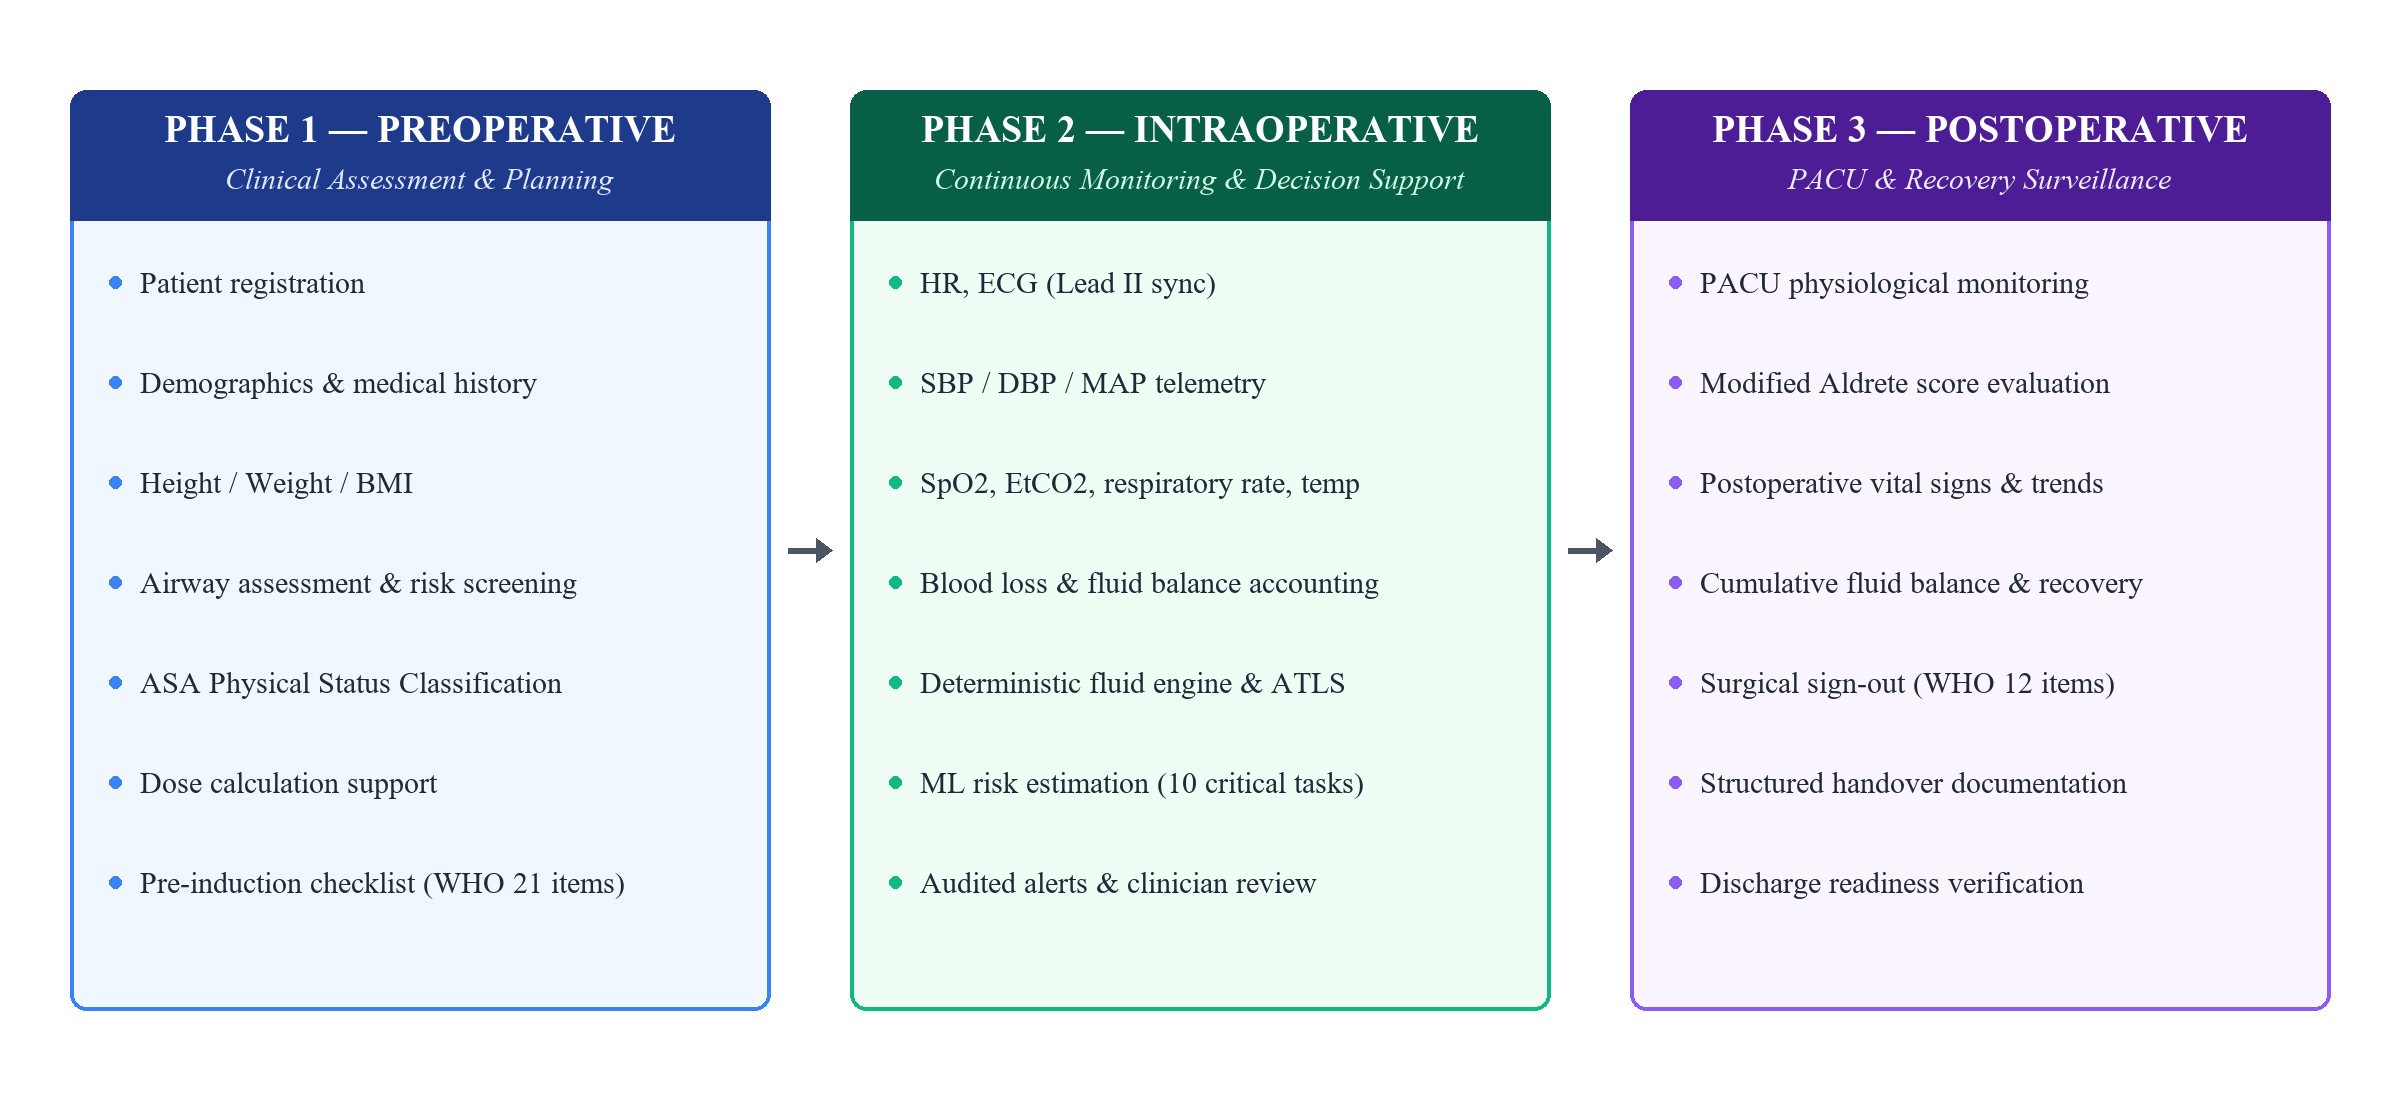
\includegraphics[width=0.74\textwidth]{figures_polished/fig2_workflow.png}
\caption{Three-phase perioperative workflow implemented in Anesth AI.}
\label{fig:workflow}
\end{figure*}

\section{Datasets and Methodology}

\subsection{Benchmark Clinical Repositories}
Anesth AI utilizes four established biomedical repositories (Table~\ref{tab:datasets}): (1) \textbf{VitalDB} (Lee et al., 2022): 6,388 surgical cases ($708,755$ time windows) comprising high-resolution arterial pressures, heart rate, $\text{SpO}_2$, capnography, and central venous pressure, utilized for Hypotension, Hypoxia, Bradycardia, and Tachycardia; (2) \textbf{MIT-BIH Arrhythmia Database} (Goldberger et al., 2000): 48 two-channel ambulatory Holter ECG recordings sampled at 360~Hz with physician-annotated heartbeat labels ($109,494$ beats), utilized for Arrhythmia Detection; (3) \textbf{MIMIC-IV-ED v2.2} (Johnson et al., 2023): $425,087$ emergency encounters across $205,504$ unique patients, utilized for Emergency Severity Assessment; and (4) \textbf{MIMIC-IV In-Hospital v3.1} (Johnson et al., 2023): $299,712$ hospital admissions comprising laboratory measurements, fluid administrations, transfusion records, and inpatient outcomes, utilized for Blood Loss, Fluid Recommendation, ICU Admission, and Mortality.

\begin{table*}[t]
\centering
\caption{Dataset and Preprocessing Summary}
\label{tab:datasets}
\begin{tabularx}{\textwidth}{l l l l X}
\toprule
\textbf{Dataset} & \textbf{Modality} & \textbf{Cohort} & \textbf{Tasks} & \textbf{Key Preprocessing} \\
\midrule
\textbf{VitalDB} & High-frequency telemetry & 6,388 cases (708,755 windows) & Hypotension, Hypoxia, Bradycardia, Tachycardia & Backward rolling stats ($t-300\text{s}$ to $t$); purged target blood pressure, $\text{SpO}_2$, and HR. \\
\textbf{MIT-BIH} & Dual-channel ECG (360 Hz) & 48 records (109,494 beats) & Arrhythmia Detection & Pan-Tompkins QRS alignment; 360-sample windows; record-independent 34/7/7 split. \\
\textbf{MIMIC-IV-ED} & Emergency Department EHR & 425,087 encounters (205,504 pts) & Emergency Severity & Target-defining acuity purged; median imputation on train; CatBoost ordered encoding. \\
\textbf{MIMIC-IV} & Inpatient EHR \& Lab events & 299,712 hospital admissions & Blood Loss, Fluid Rec., ICU Adm., Mortality & Post-event labs \& LOS purged; sequential padding (seq\_len=24); train-only StandardScaler. \\
\bottomrule
\end{tabularx}
\end{table*}

\subsection{Rigorous Leakage Prevention Protocol}
To ensure scientific validity, a strict leakage prevention protocol was enforced across all tasks: (1) \textit{Patient/Record-Grouped Partitioning:} Data was partitioned into training ($70\%$), validation ($15\%$), and frozen test ($15\%$) cohorts strictly grouped by patient or record identifiers (caseid in VitalDB, subject\_id in MIMIC-IV and MIMIC-IV-ED, and record\_id in MIT-BIH), enforcing zero patient overlap such that $P_{\text{train}} \cap P_{\text{val}} = \emptyset$ and $P_{\text{train}} \cap P_{\text{test}} = \emptyset$; (2) \textit{Target-Defining Feature Purging:} Features that directly define target outcomes were permanently removed: arterial blood pressures purged from Hypotension; continuous $\text{SpO}_2$ purged from Hypoxia; heart rate indicators purged from Bradycardia and Tachycardia; triage acuity scores purged from Emergency Severity; and post-admission laboratory measurements and length-of-stay metrics purged from inpatient models; (3) \textit{Train-Only Preprocessing Parameter Fitting:} Imputation medians and feature normalization scalers were computed exclusively on training partitions and applied without modification to validation and test partitions; (4) \textit{Pre-Outcome Backward Rolling Windows:} Intraoperative time series summary statistics were computed backward across a 5-minute window [$t - 300\text{s}$, $t$], precluding lookahead leakage; and (5) \textit{Single-Touch Frozen Evaluation:} Test partitions remained completely untouched during model development; thresholds were selected and locked on validation Precision-Recall curves before single-touch evaluation on frozen test sets.

\subsection{Operational Prediction Architectures}
The comparative evaluation framework benchmarks multiple algorithms across distinct learning paradigms, selecting the champion architecture for each prediction task: \textit{HistGradientBoosting} with native missing value handling and fast inference for Hypotension, Hypoxia, and Tachycardia; \textit{LightGBM} (Ke et al., 2017) providing leaf-wise tree growth, exact TreeSHAP attribution compatibility, and strong probability calibration for Arrhythmia Detection and Fluid Recommendation; \textit{CatBoost} (Prokhorenkova et al., 2018) with symmetric trees and ordered target encoding for high-cardinality categorical triage features in Emergency Severity Assessment; \textit{ClinicalCNN (1D-CNN)} comprising three convolutional blocks (filters 64--128, kernel sizes 3, 5) with batch normalization, max pooling, and dropout ($0.25$) for Bradycardia; \textit{ClinicalLSTM} featuring a two-layer bidirectional LSTM (hidden dimension 64, dropout $0.20$) for Surgical Blood Loss; and \textit{ClinicalGRU} featuring a two-layer Gated Recurrent Unit network (hidden dimension 64, dropout $0.20$) for sequential learning on ICU Admission and In-Hospital Mortality. Demonstration modules (Airway, RiskPrediction, PONV, PACU, DrugSafety) are maintained strictly as non-validated prototypes and excluded from scientific claims.

\section{Clinical Calculation and Safety Support}

\subsection{Anesthesia Dose Calculation Decision Support}
Pharmacological dose support in Anesth AI provides deterministic, parameter-driven guidance based on patient-specific physiological indicators: (1) Total Body Weight ($\text{TBW} = \text{measured body weight in kg}$); (2) Body Mass Index ($\text{BMI} = \text{Weight} / \text{Height}^2$); (3) Lean Body Mass (LBM) computed via the Janmahasatian formulation (Janmahasatian et al., 2005; Eleveld et al., 2018):
\begin{align}
\text{LBM}_{\text{Male}} &= \frac{9270 \times W}{6680 + (216 \times \text{BMI})} \\
\text{LBM}_{\text{Female}} &= \frac{9270 \times W}{8780 + (244 \times \text{BMI})}
\end{align}
(4) Physiological scaling adjustments for age-related clearance reductions in geriatric cohorts ($\ge 65$ years); and (5) Organ function screening flags for severe aortic stenosis, renal impairment, and hepatic insufficiency. The workflow evaluates patient body size and determines whether TBW or LBM serves as the relevant dosing basis: Patient data $\rightarrow$ TBW/BMI $\rightarrow$ LBM where applicable $\rightarrow$ dosing basis $\rightarrow$ configured calculation $\rightarrow$ safety checks $\rightarrow$ clinician review $\rightarrow$ documented recommendation (Fig.~\ref{fig:dose}). The module provides decision support; it does not autonomously prepare or administer medications. Specific drug dosing parameters not provided in verified project references remain under attending clinician determination.

\begin{figure}[t]
\centering
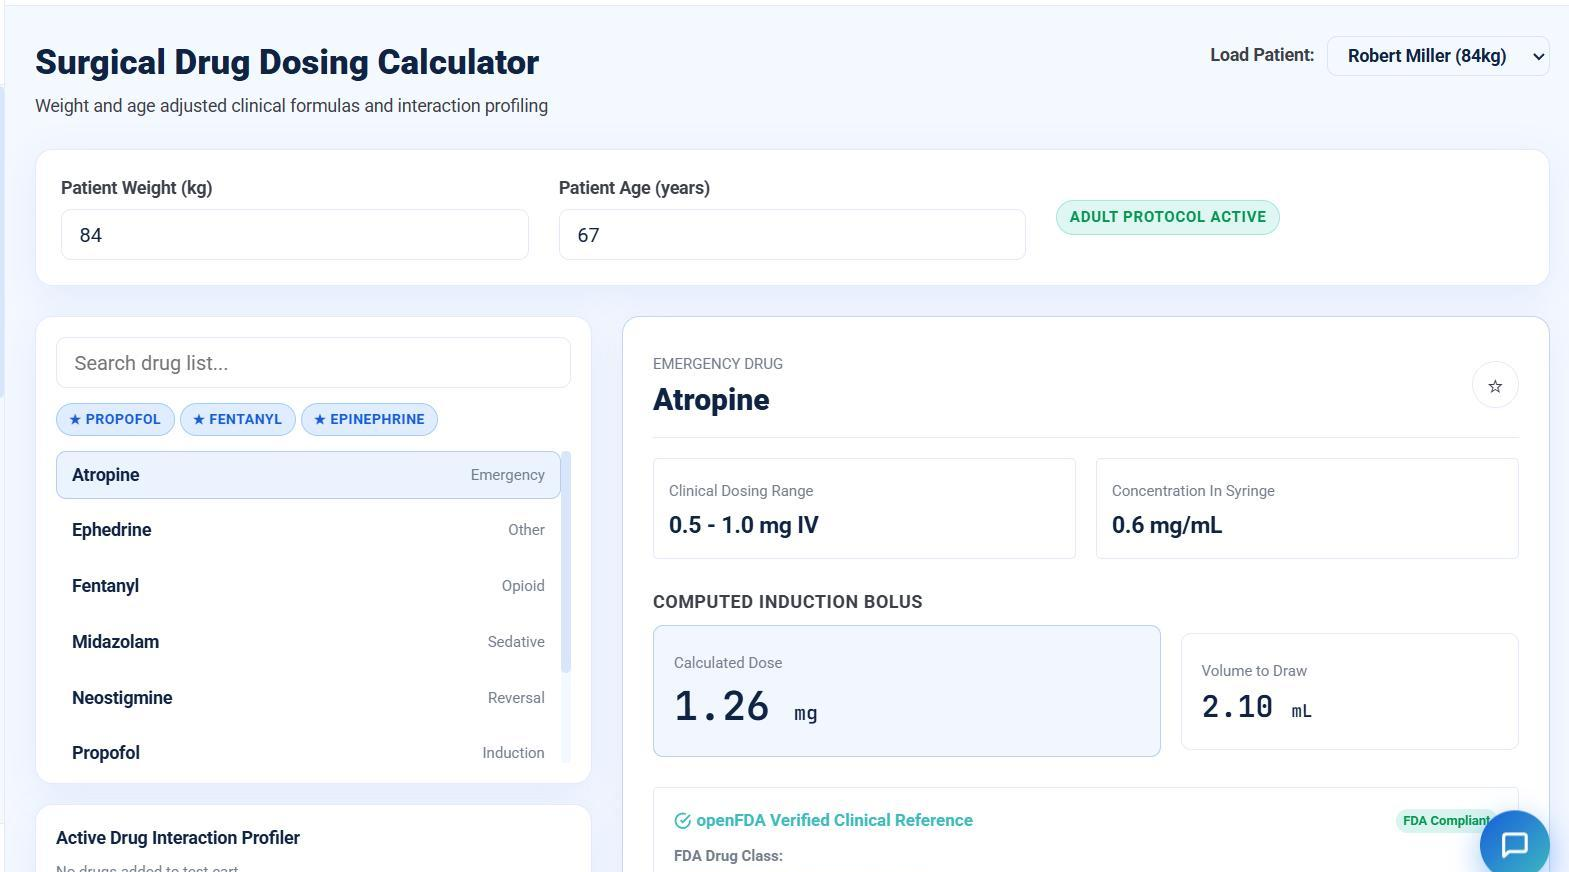
\includegraphics[width=0.82\columnwidth]{figures_polished/fig3_dose_calculator.png}
\caption{Anesth AI anesthesia dose-calculation decision-support interface.}
\label{fig:dose}
\end{figure}

\subsection{Deterministic Physiological Fluid Engine}
Intraoperative fluid management requires transparent physiological accounting rather than opaque machine learning regression. Anesth AI completely decouples: (1) \textit{Statistical ML Fluid Recommendation:} A validated LightGBM classifier predicting the empirical probability that similar patient profiles received intravenous fluid boluses; and (2) \textit{Deterministic Physiological Fluid Engine:} An arithmetic service executing authoritative physiological formulas:

\textit{1) Holliday-Segar Maintenance Rate ($R$ in mL/hr):} For $W \le 10\text{ kg}$, $R = 4W$; for $10 < W \le 20\text{ kg}$, $R = 40 + 2(W - 10)$; for $W > 20\text{ kg}$, $R = 60 + (W - 20)$ (Holliday and Segar, 1957). The Holliday-Segar calculation is presented as a basal/reference calculation and not as a universal intraoperative fluid prescription; third-space replacement formulas are deliberately omitted.

\textit{2) Cumulative Fluid Input ($F_{\text{in}}$):} $F_{\text{in}} = \text{Crystalloids} + \text{Colloids} + \text{Blood Products} + \text{Other documented IV inputs}$.

\textit{3) Cumulative Measured Fluid Losses ($F_{\text{loss}}$):} $F_{\text{loss}} = \text{Blood Loss} + \text{Urine Output} + \text{Drain/Suction Losses} + \text{Other measured losses}$.

\textit{4) Net Fluid Balance:} $\text{Net Balance} = F_{\text{in}} - F_{\text{loss}}$; $\text{Normalized Net Balance} = \text{Net Balance} / \text{Weight}$ (mL/kg).

\textit{5) Urine Output Rate:} $\text{UO}_{\text{rate}} = \text{Urine Volume} / (\text{Weight} \times \text{Duration})$ in mL/kg/hr.

\textit{6) Estimated Blood Volume (EBV):} $\text{EBV} = \text{Weight} \times 70\text{ mL/kg}$ (Male), $\text{Weight} \times 65\text{ mL/kg}$ (Female) (ATLS, 2018).

\textit{7) Blood Loss Percentage:} $\text{Blood Loss \%} = (\text{Measured Blood Loss} / \text{EBV}) \times 100$, mapped to configured ATLS hemorrhage classes (Classes I--IV).

\textit{8) Documented Safety Flags:} Excessive positive fluid balance ($>30\text{ mL/kg}$ or $>2500\text{ mL}$), sustained oliguria ($<0.5\text{ mL/kg/hr}$ for $>1\text{ hr}$ as defined by KDIGO, 2012), significant surgical hemorrhage ($>15\%\text{ EBV}$), and ATLS Class III/IV shock. These triggers operate strictly as decision-support safety flags and not automatic treatment commands. The system does not autonomously administer or titrate fluids.

\begin{figure}[t]
\centering
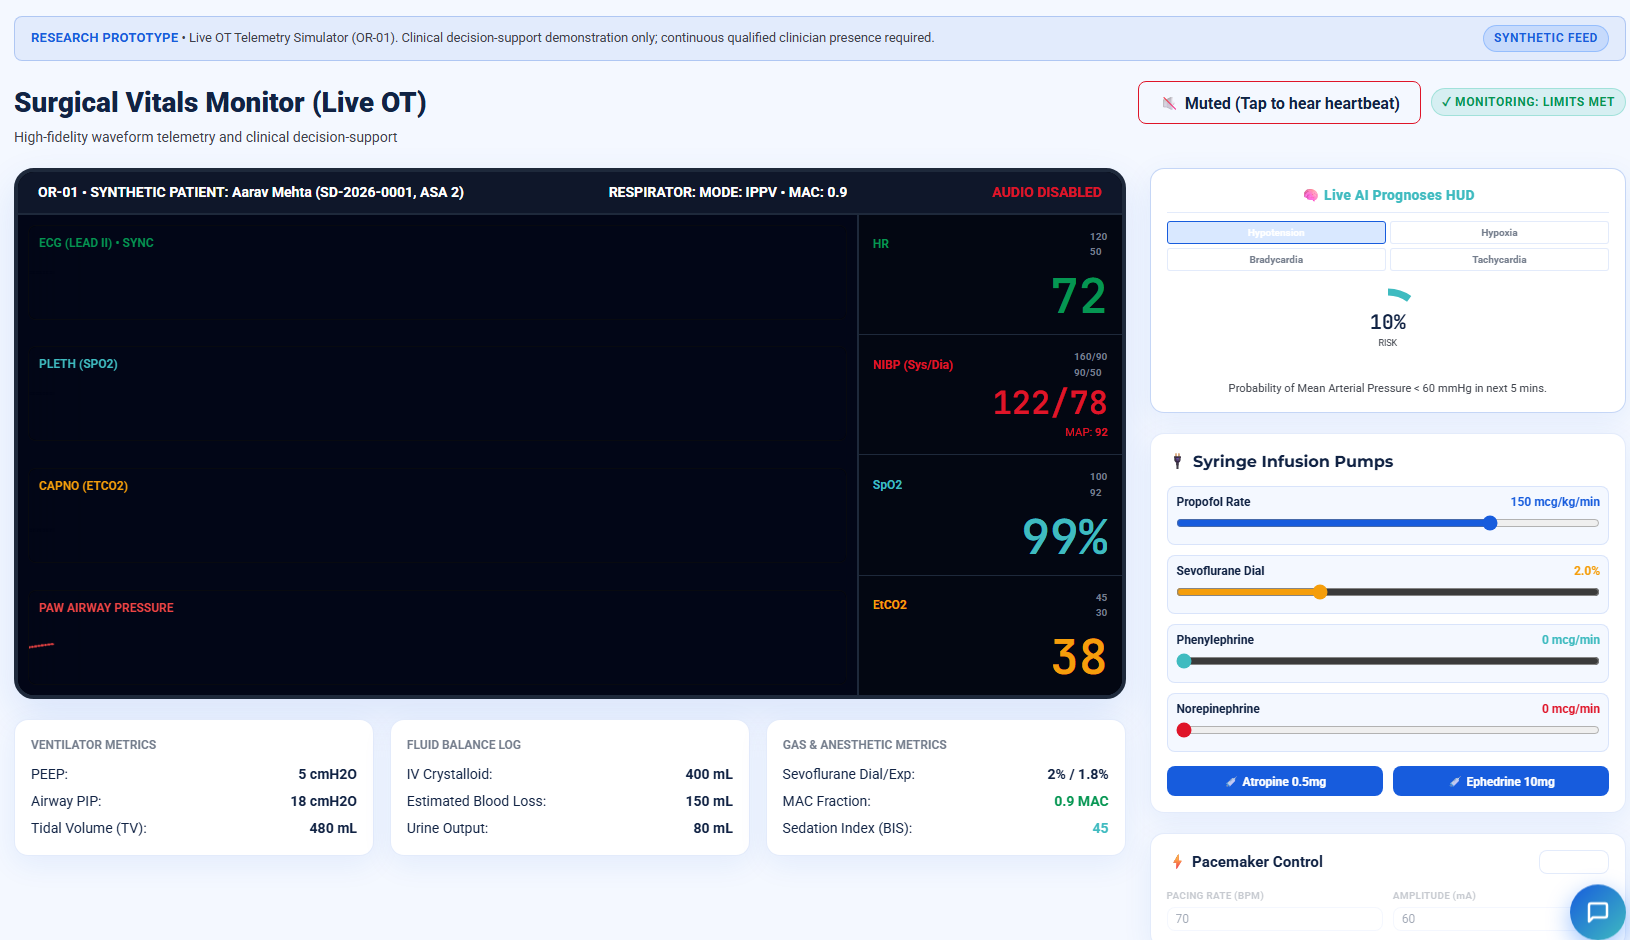
\includegraphics[width=0.82\columnwidth]{figures_polished/fig4_live_ot.png}
\caption{Live operating theatre telemetry and clinical decision-support interface of Anesth AI.}
\label{fig:live_ot}
\end{figure}

\subsection{Clinician-Confirmed ASA Physical Status Classification}
In adherence to American Society of Anesthesiologists standards (ASA, 2020), Anesth AI strictly enforces the standardized terminology: \textbf{ASA Physical Status Classification} (ASA I through ASA VI): ASA I (Normal healthy patient), ASA II (Mild systemic disease), ASA III (Severe systemic disease), ASA IV (Severe systemic disease that is a constant threat to life), ASA V (Moribund patient not expected to survive without the operation), and ASA VI (Declared brain-dead organ donor). Emergency case status is recorded as an independent clinical toggle: \textbf{Emergency Case: Yes/No}. When affirmed, modifier ``E'' is appended (e.g., ASA III-E). Automated AI assignment of ASA status is prohibited; the attending clinician selects and confirms the classification with provider credentials, timestamp, and clinical justification.

\subsection{Intraoperative Alert Semantics and Surgical Checklists}
The telemetry module monitors HR, SBP, DBP, MAP, $\text{SpO}_2$, RR, $\text{EtCO}_2$, and temperature (Fig.~\ref{fig:live_ot}). To prevent false clinical complacency, nominal monitoring states explicitly state: \textit{``Monitoring status: No configured alerts currently triggered.''} Generic or unqualified declarations of safety are strictly prohibited. When an alert triggers, it details the affected parameter, current value, trend direction, severity level, potential clinical causes, recommended verification checks, and logs clinician acknowledgment or override rationale into the immutable audit trail. Conforming to WHO guidelines (WHO, 2009), the system enforces structured verification: Pre-Induction Checklist (21 safety items) and Surgical Sign-Out Checklist (12 items).

\section{Experimental Results}
The ten operational clinical prediction tasks were systematically evaluated on untouched, patient-independent held-out cohorts under zero-leakage protocols. Table~\ref{tab:results} summarizes performance across all ten tasks.

\begin{table*}[t]
\centering
\caption{Ten Clinical Prediction Task Performance Across Benchmark Frozen Test Cohorts}
\label{tab:results}
\begin{tabularx}{\textwidth}{l l l c c c c c c c c c}
\toprule
\textbf{Task} & \textbf{Dataset} & \textbf{Model} & \textbf{Test Cohort} & \textbf{Positives} & \textbf{Thresh.} & \textbf{Accuracy} & \textbf{Sens.} & \textbf{Spec.} & \textbf{Prec.} & \textbf{F1} & \textbf{ROC-AUC} \\
\midrule
Hypotension & VitalDB & HistGradBoost & 708,755 & 173,859 & 0.475 & 69.88\% & 54.14\% & 75.00\% & 41.31\% & 46.86\% & 0.6974 \\
Hypoxia & VitalDB & HistGradBoost & 708,755 & 6,986 & 0.825 & 98.67\% & 48.47\% & 99.16\% & 36.62\% & 41.72\% & 0.9047 \\
Bradycardia & VitalDB & ClinicalCNN & 708,755 & 82,753 & 0.600 & 77.48\% & 28.73\% & 83.93\% & 19.11\% & 22.95\% & 0.6448 \\
Tachycardia & VitalDB & HistGradBoost & 708,755 & 95,832 & 0.250 & 67.73\% & 62.11\% & 68.60\% & 23.62\% & 34.23\% & 0.6980 \\
Arrhythmia & MIT-BIH & LightGBM & 17,029 & 5,843 & 0.220 & 85.62\% & 92.01\% & 82.29\% & 73.07\% & 81.45\% & 0.9414 \\
Emerg. Severity & MIMIC-ED & CatBoost & 64,375 & 25,299 & 0.325 & 53.98\% & 78.78\% & 37.92\% & 45.10\% & 57.37\% & 0.6657 \\
Blood Loss & MIMIC-IV & ClinicalLSTM & 82,204 & 19,200 & 0.525 & 76.65\% & 70.82\% & 78.43\% & 50.01\% & 58.62\% & 0.8349 \\
Fluid Rec. & MIMIC-IV & LightGBM & 82,204 & 28,982 & 0.525 & 78.33\% & 78.65\% & 78.15\% & 66.22\% & 71.90\% & 0.8687 \\
ICU Admission & MIMIC-IV & ClinicalGRU & 82,204 & 34,037 & 0.425 & 77.87\% & 85.98\% & 72.14\% & 68.56\% & 76.29\% & 0.8814 \\
Mortality & MIMIC-IV & ClinicalGRU & 82,204 & 1,822 & 0.900 & 97.38\% & 26.34\% & 98.99\% & 37.12\% & 30.82\% & 0.8663 \\
\bottomrule
\end{tabularx}
\end{table*}

\subsection{Calibration \& Arrhythmia Revalidation}
Probability calibration was evaluated via Brier score: Hypotension (0.1924), Hypoxia (0.0338), Bradycardia (0.2037), Tachycardia (0.1353), Arrhythmia (0.0613), Emergency Severity (0.2137), Blood Loss (0.1617), Fluid Recommendation (0.1492), ICU Admission (0.1413), and Mortality (0.1356). For Arrhythmia, Balanced Accuracy was 87.15\% and PR-AUC was 0.9494.

An earlier annotation parsing issue was corrected by parsing all 48 MIT-BIH records (109,494 beats: 75,052 Normal, 34,442 Arrhythmia) under a strict record-independent split: 34 train, 7 val, 7 frozen test records (102, 103, 200, 210, 213, 217, 220; 17,029 beats: 11,186 normal, 5,843 arrhythmia). The LightGBM model detected 5,376 of 5,843 arrhythmias (Table~\ref{tab:cm}).

\begin{table}[h]
\centering
\caption{MIT-BIH Arrhythmia Confusion Matrix ($N = 17,029$)}
\label{tab:cm}
\begin{tabular}{lccc}
\toprule
\textbf{Actual \textbackslash\ Predicted} & \textbf{Pred. Normal} & \textbf{Pred. Arrhythmia} & \textbf{Total} \\
\midrule
\textbf{Actual Normal} & 9,202 (TN) & 1,981 (FP) & 11,186 \\
\textbf{Actual Arrhythmia} & 467 (FN) & 5,376 (TP) & 5,843 \\
\midrule
\textbf{Total} & 9,669 & 7,357 & 17,029 \\
\bottomrule
\end{tabular}
\end{table}

\begin{figure}[t]
\centering
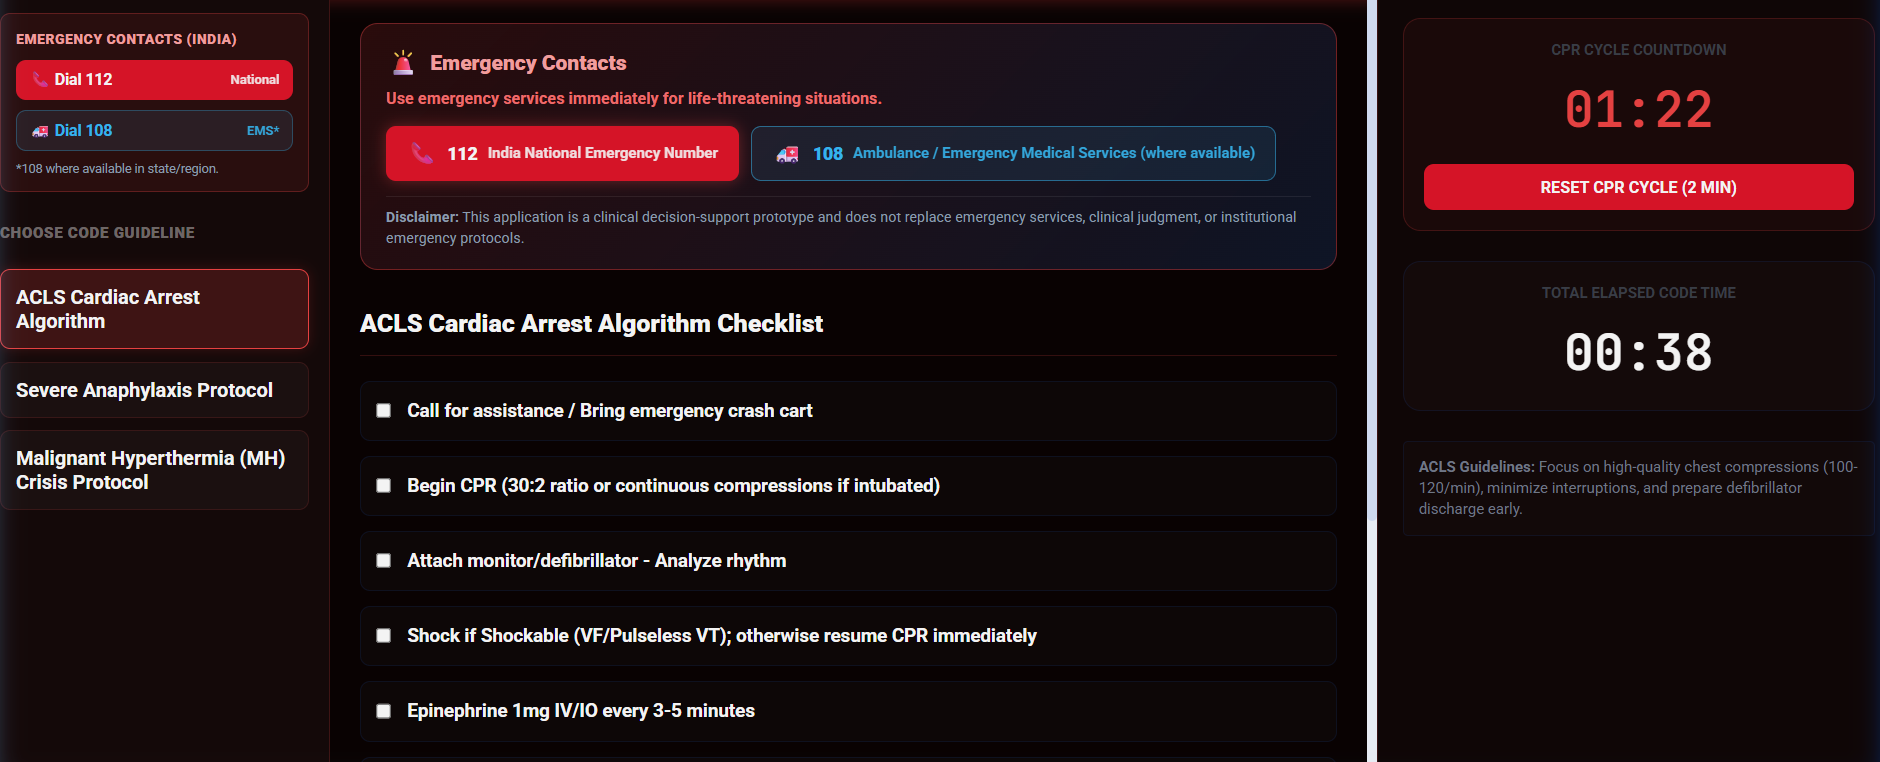
\includegraphics[width=0.80\columnwidth]{figures_polished/fig5_emergency.png}
\caption{Emergency Break-Glass access interface with audited emergency access controls.}
\label{fig:emergency}
\end{figure}

\subsection{Dual-Tier RBAC and Emergency Break-Glass}
Centralized RBAC across six roles using HMAC-SHA256 JWT tokens is paired with audited Emergency Break-Glass access (Fig.~\ref{fig:emergency}): active clinician auth required (HTTP 401), mandatory clinical rationale $\ge 10$ chars (HTTP 422), temporary scoped JWT (15--60 min), and immutable audit logs. Advisory numbers: \textbf{112} (India National Emergency) and \textbf{108} (Ambulance/EMS). No automatic dispatch is claimed.

\section{Safety, Limitations and Future Work}
\textbf{Human-in-the-Loop Safety:} Anesth AI does not autonomously administer drugs, titrate anesthesia, administer fluids, modify ventilator settings, or assign ASA status. The system does not replace anesthesiologists; ML outputs are advisory decision support under clinician oversight.

\textbf{Limitations:} Retrospective cohorts; telemetry domain shift (ambulatory Holter vs. surgical electrocautery); low-prevalence outcome sensitivity; prototype status without prospective trials; mandatory continuous clinician supervision.

\textbf{Future Work:} Prospective high-fidelity simulation with certified anesthesiologists; multi-center operating room validation; HL7/FHIR streaming integration; conformal uncertainty quantification.

\section{Conclusion}
In this paper, we presented \textbf{Anesth AI}, an integrated, human-in-the-loop clinical decision-support prototype for personalized anesthesia management and patient safety. By evaluating ten operational prediction tasks across VitalDB, MIT-BIH, MIMIC-IV-ED, and MIMIC-IV, the framework demonstrates unified perioperative risk modeling. Enforcing patient-grouped splitting, eliminating target-defining variables, and resolving the Arrhythmia evaluation artifact, Anesth AI establishes a scientifically rigorous benchmark while decoupling statistical ML from deterministic fluid accounting under clinician oversight.

\begin{thebibliography}{00}

\bibitem{ref1}
K.~Shimada \textit{et al.}, ``Artificial Intelligence-Assisted Interventions for Perioperative Anesthetic Management: A Systematic Review and Meta-Analysis,'' \textit{BMC Anesthesiology}, vol.~24, no.~1, pp.~112--124, 2024.

\bibitem{ref2}
Z.~Hu, G.~Pan, X.~Wang, and K.~Li, ``Intelligent Algorithm Based on Deep Learning to Predict the Dosage for Anesthesia,'' \textit{Computer Methods and Programs in Biomedicine}, vol.~244, p.~107982, 2024.

\bibitem{ref3}
Y.~Shu \textit{et al.}, ``Applications of Artificial Intelligence in Anesthesiology: Current Trends and Future Perspectives,'' \textit{Journal of Clinical Anesthesia}, vol.~99, p.~111652, 2025.

\bibitem{ref4}
M.~Fei \textit{et al.}, ``Artificial Intelligence in Anesthesia and Perioperative Medicine: A Review of Clinical Decision Support and Patient Safety,'' \textit{Frontiers in Medicine}, vol.~12, p.~1421098, 2025.

\bibitem{ref5}
M.~Bellini \textit{et al.}, ``Clinical Decision Support Systems in Perioperative Medicine: Implementation, Efficacy, and Safety Governance,'' \textit{British Journal of Anaesthesia}, vol.~134, no.~2, pp.~210--223, 2025.

\bibitem{ref6}
D.~Chae, S.~H.~Park, and T.~Lee, ``Multi-Modal Physiological Telemetry and Deep Sequence Modeling for Intraoperative Risk Prediction,'' \textit{IEEE Transactions on Biomedical Engineering}, vol.~73, no.~1, pp.~145--156, 2026.

\bibitem{ref7}
T.~Lee \textit{et al.}, ``VitalDB, a High-Fidelity Multi-Parameter Vital Signs Database in Surgical Patients,'' \textit{Scientific Data}, vol.~9, no.~1, p.~279, 2022.

\bibitem{ref8}
A.~L.~Goldberger \textit{et al.}, ``PhysioBank, PhysioToolkit, and PhysioNet: Components of a New Research Resource for Complex Physiologic Signals,'' \textit{Circulation}, vol.~101, no.~23, pp.~e215--e220, 2000.

\bibitem{ref9}
A.~E.~W.~Johnson \textit{et al.}, ``MIMIC-IV, a Freely Accessible Electronic Health Record Dataset,'' \textit{Scientific Data}, vol.~10, no.~1, p.~1, 2023.

\bibitem{ref10}
A.~E.~W.~Johnson \textit{et al.}, ``MIMIC-IV-ED, Emergency Department Module,'' \textit{PhysioNet}, 2023.

\bibitem{ref11}
M.~A.~Holliday and W.~E.~Segar, ``The Maintenance Need for Water in Parenteral Fluid Therapy,'' \textit{Pediatrics}, vol.~19, no.~5, pp.~823--832, 1957.

\bibitem{ref12}
American College of Surgeons Committee on Trauma, \textit{Advanced Trauma Life Support (ATLS) Student Course Manual}, 10th~ed., Chicago, IL, 2018.

\bibitem{ref13}
American Society of Anesthesiologists, ``ASA Physical Status Classification System,'' ASA House of Delegates Standards, 2020.

\bibitem{ref14}
World Health Organization, \textit{WHO Guidelines for Safe Surgery 2009: Safe Surgery Saves Lives}, World Health Organization, Geneva, 2009.

\bibitem{ref15}
KDIGO Work Group, ``KDIGO Clinical Practice Guideline for Acute Kidney Injury,'' \textit{Kidney International Supplements}, vol.~2, no.~1, pp.~1--138, 2012.

\bibitem{ref16}
D.~J.~Eleveld \textit{et al.}, ``Pharmacokinetic-Pharmacodynamic Model for Propofol for Broad Patient Populations,'' \textit{Anesthesiology}, vol.~128, no.~5, pp.~882--894, 2018.

\bibitem{ref17}
S.~Janmahasatian \textit{et al.}, ``Quantification of Lean Bodyweight,'' \textit{Clinical Pharmacokinetics}, vol.~44, no.~10, pp.~1051--1065, 2005.

\bibitem{ref18}
G.~Ke \textit{et al.}, ``LightGBM: A Highly Efficient Gradient Boosting Decision Tree,'' \textit{Advances in Neural Information Processing Systems (NeurIPS)}, vol.~30, pp.~3146--3154, 2017.

\bibitem{ref19}
L.~Prokhorenkova \textit{et al.}, ``CatBoost: Unbiased Boosting with Categorical Features,'' \textit{Advances in Neural Information Processing Systems (NeurIPS)}, vol.~31, pp.~6638--6648, 2018.

\end{thebibliography}

\end{document}
